% 图 6.1 压杆屈曲：载荷 100/200/300 kg，(c)(d) S 形屈曲互为镜像
\documentclass[tikz,border=5pt]{standalone}
\usetikzlibrary{arrows.meta,patterns}
\usepackage{amsmath}
\usepackage{bm}
\usepackage{fontspec}
\setmainfont{Times New Roman}
\begin{document}
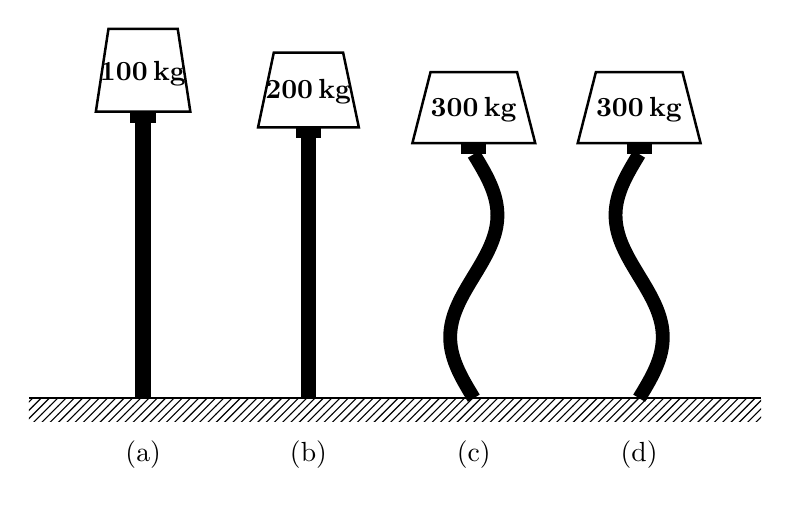
\begin{tikzpicture}[line width=0.8pt,>=Stealth]
% ---- panel macro-ish drawing ----
% (a) 100 kg, straight rod
\draw[line width=5.5pt] (0.9,0) -- (0.9,3.5);
\fill (0.74,3.5) rectangle (1.06,3.64);
\draw[fill=white,line width=0.9pt] (0.30,3.64) -- (1.50,3.64) -- (1.34,4.69) -- (0.46,4.69) -- cycle;
\node at (0.9,4.12) {\textbf{100\,kg}};
% (b) 200 kg, shorter straight rod, wider weight
\draw[line width=5.5pt] (3.0,0) -- (3.0,3.3);
\fill (2.84,3.3) rectangle (3.16,3.44);
\draw[fill=white,line width=0.9pt] (2.36,3.44) -- (3.64,3.44) -- (3.44,4.39) -- (2.56,4.39) -- cycle;
\node at (3.0,3.9) {\textbf{200\,kg}};
% (c) 300 kg, buckled S (upper bulge right, lower bulge left)
\draw[line width=5pt] plot[domain=0:3.1,samples=41,smooth]
  ({5.1-0.30*sin(360*\x/3.1)},{\x});
\fill (4.94,3.1) rectangle (5.26,3.24);
\draw[fill=white,line width=0.9pt] (4.32,3.24) -- (5.88,3.24) -- (5.65,4.14) -- (4.55,4.14) -- cycle;
\node at (5.1,3.67) {\textbf{300\,kg}};
% (d) 300 kg, mirrored buckling
\draw[line width=5pt] plot[domain=0:3.1,samples=41,smooth]
  ({7.2+0.30*sin(360*\x/3.1)},{\x});
\fill (7.04,3.1) rectangle (7.36,3.24);
\draw[fill=white,line width=0.9pt] (6.42,3.24) -- (7.98,3.24) -- (7.75,4.14) -- (6.65,4.14) -- cycle;
\node at (7.2,3.67) {\textbf{300\,kg}};
% ---- shared hatched ground ----
\fill[pattern=north east lines] (-0.55,-0.3) rectangle (8.75,0);
\draw[line width=0.9pt] (-0.55,0) -- (8.75,0);
% ---- panel labels ----
\node at (0.9,-0.72) {(a)};
\node at (3.0,-0.72) {(b)};
\node at (5.1,-0.72) {(c)};
\node at (7.2,-0.72) {(d)};
\end{tikzpicture}
\end{document}
